
\chapter{Sistemas HAR }

\label{chap4:sistemas-de-reconocimiento}

\section{Introducción}

\label{sec41:introduccion}El diseño de sistemas con conocimiento
del contexto promueven una interacción novedosa con los usuarios y
diversas aplicaciones en las áreas de ambientes inteligentes, repuesta
a emergencias, vigilancia y otros \cite{Choudhury2008}. Un sistema
con la capacidad de reconocer las actividades humanas por medio del
uso de sensores empotrados posee mecanismos para crear aplicaciones
de cuidado personal, salud y asistencia inteligente. El requerimiento
primordial de un sistema con una aplicación de contexto es que este
pueda ser portado continuamente como atuendo de sus usuarios (un sistema
\abbr{Wearable}). Por lo tanto, un sistema que acompaña continuamente
al usuario puede interaccionar oportunamente con el mismo ya que este
tiene la capacidad de observar en tiempo real las acciones de su portador.
La ventaja adicional de un sistema de este tipo es que puede ser desactivado
fácilmente o removido de la actividad diaria de su usuario.

En este capítulo se definen los componentes principales de un sistema
de reconocimiento de actividades humanas (sistemas \abbr{HAR}). El
objetivo principal del sistema \abbr{HAR}en conjunto es proveer módulo
base para aplicaciones novedosas de contexto. El módulo debe ser capaz
de reconocer varias actividades realizadas rutinariamente de diferentes
maneras, por diferentes usuarios y en diferentes condiciones contextuales.
Las funciones principales de los componentes descritos en la primera
sección exponen los mecanismos para implementar los mismos en base
trabajos relacionados de \abbr{HAR} \cite{Choudhury2008,ReyesOrtiz2015}. 

La última sección, enumera los requisitos no funcionales para lograr
una aplicación de contexto móvil y ubicua. Por un lado, las características
esperadas en una aplicación de esta naturaleza, y por el otro los
requisitos técnicos de los dispositivos móviles y los sensores empotrados
utilizados como hardware de implementación.

\section{Arquitectura del sistema}

\label{sec42:componentes}El diseño de la arquitectura de componentes
de un sistema \abbr{HAR} se rige de acuerdo a las guías de implementación
de una aplicación de aprendizaje automático (\abbr{ML}). De acuerdo
al proceso definido en la sección \ref{sec262:proceso-har}, se tiene
en cuenta la misma estructura de componentes y las mismas fases de
procesamiento de información. Además, se debe contemplar que el proceso
se divide en dos etapas: la etapa de entrenamiento y la de evaluación
\cite{LaraLabrador2013}. 

Ambas etapas requieren la implementación de los mismos componentes,
pero un sistema \abbr{HAR} práctico debe contemplar principalmente
la fase de evaluación, ya que el reconocimiento de actividades resulta
de una \emph{predicción} basado en un algoritmo de \abbr{ML} en-linea
(\emph{On-line learning}). Sin embargo, la etapa de entrenamiento
es un elemento clave para el sistema ya que es el punto de partida
para el \emph{aprendizaje} basado en modelo de \abbr{ML} y usualmente
se realiza bajo demanda (\emph{Off-line learning}).

Bajo el marco teórico de los sistemas \abbr{HAR} basados en \abbr{ML},
se han identificado unos componentes comunes para realizar las funcionalidades
de aprendizaje y predicción según\cite{Choudhury2008}. Un sistema
de reconocimiento de actividades posee tres componentes:
\begin{itemize}
\item un \emph{recolector }de medidas
\item un\emph{ procesador }de muestras 
\item un \emph{clasificador }de actividades
\end{itemize}
En la \figref{fig42:componentes-har} se muestra una vista general
de los componentes y sus interrelaciones. Las funcionalidades de cada
componente se describen a continuación. 

\begin{figure}[!tbph]
\centering{}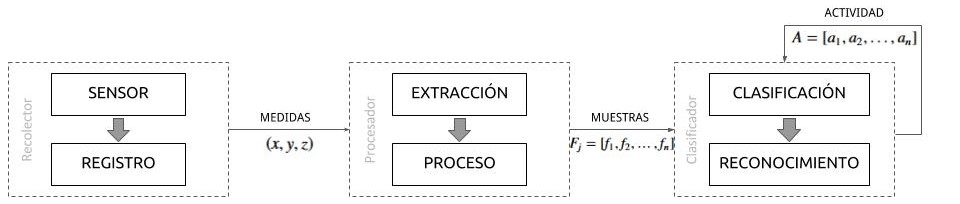
\includegraphics[width=1\linewidth]{capitulo-4/graphics/diagrama_4_1}\caption{Componentes de los sistemas \abbr{HAR}}
\label{fig42:componentes-har}
\end{figure}


\subsection{Recolector de medidas}

\label{sec421:recolector-datos}El recolector de datos tiene la función
de capturar medidas de los sensores e registrar la información indexada
en la dimensión del tiempo. La captura de datos relevantes para los
sistemas \abbr{HAR} debe ser realizada con instrumentos de medición
apropiados: en nuestro caso con sensores (\abbr{Wearables})\ref{sec23:sensores}.
Los sensores empotrados se utilizan para recolectar señales directamente
de los usuarios. Estos deben estar anexados al cuerpo como la cintura,
la muñeca, el pectoral, los muslos o la cabeza \cite{Bao2004}, también
pueden ser portados simplemente ya están comúnmente empotrados en
dispositivos de uso regular como los teléfonos móviles modernos, relojes
o lentes inteligentes \cite{LaraLabrador2012,Choudhury2008}.

\subsubsection{Registro}

Las señales de variables medidas deben ser registrados de manera secuencial
y transmitidos para su posterior procesamiento.

\subsubsection{Señales de Aceleración}

\subsubsection{Señales de Giroscopio}

\subsubsection{Señales de Ubicación}

\subsubsection{Señales de Fisiológicas}

\subsection{Procesador de muestras}

\label{sec422:proceso-se=0000F1ales}Proceso de señales en bruto para
adecuarlos muestras con variables significativas que permitan discriminar
las actividades a reconocer

\subsubsection{Etiquetado}

\subsubsection{Filtro de Señal}

\subsubsection{Muestreo}

\subsection{Clasificador de actividades}

\label{sec423:clasificador}Utiliza las muestras extraídas para construir
un modelo e predecir qué actividad probable está realizando un individuo
en un determinado instante.

\subsubsection{Clasificación}

\subsubsection{Reconocimiento}

\section{Capacidades deseables}

\subsection{Características no funcionales}

\label{sec431:caracteristicas}Existen un conjunto de características
deseables que deben ser satisfechas para la construcción efectiva
de los sistemas de reconocimiento. Estas características abordan cuestiones
de diseño importantes que conciernen a la calidad y al funcionamiento
del sistema:
\begin{enumerate}
\item Portabilidad, el sistema utiliza sensores adjuntos a los individuos
(Ej. el acelerómetro) y no deben obstruir las actividades cotidianas
de los usuarios durante su uso. El fin es de evitar que se afecte
la adopción masiva del sistema. 
\item Conectividad, el sistema debe transmitir de manera confiable los datos
recolectados y/o procesados a algún componente desplegado de forma
remota. 
\item Almacenamiento, el sistema debe persistir los datos recolectados y/o
procesados de manera local en el dispositivo móvil con el fin de mantener
la calidad y minimizar la cantidad transferida a otros componentes.
\item Procesamiento, el sistema debe procesar y transformar los datos en
bruto para producir información relevante para el reconocimiento de
actividades.
\item Ubiquidad, el sistema debe operar en cualquier condición y contexto
en que la persona se encuentre sin interferir u obligar al usuario
a interactuar con el sistema.
\item Uso de energía, el sistema debe preservar el uso de energía en los
dispositivos móviles que están implementados. La lectura de datos,
el procesamiento y la conectividad no deben incurrir en gastos excesivos
de energía para que el sistema pueda operar.
\item Privacidad, el sistema debe mantener de manera confidencial los datos
recolectados y/o producidos durante la adopción masiva del sistema,
además de alertar sobre la utilización de datos sensibles que requieran
el consentimiento del usuario.
\end{enumerate}

\subsection{Dispositivos móviles}

\label{sec432:dispositivos-moviles}Descripción técnica de dispositivos
móviles: procesador, memoria, sensores y almacenamiento

\subsubsection{Teléfonos móviles}

\subsubsection{Relojes inteligentes}

\subsection{Sensores empotrados}

\label{sec433:sensores-empotrados}Descripción técnica de los sensores
de aceleración, variables, orientación en dispositivo, unidades de
medida, precisión vs consumo.

\subsubsection{Acelerómetro}

\subsubsection{Giroscopio}

\subsubsection{GPS/WIFI}

\section{Conclusión}

Resumen
